\chapter{verwendete Technologien}
\label{chap:verwendeteTechnologien}
\section{Multi-Wan Bonding}
Multi-Wan Bonding beschreibt, wie der Name schon sagt, das Bündeln einer Verbindung über mehrere WAN Zugänge. Im Normalfall handelt es sich beim WAN um das Internet. 
\\\\
Es werden dabei verschiedene WAN-Anbindungen wie LTE, Kabel, Glasfaser, vDSL, DSL und Satellit miteinander gekoppelt um eine ausfallsichere und schnellere Verbindung zu erhalten. Die Bandbreiten der einzelnen WAN-Anbindungen wird dabei fast summiert. 

\subsection{Einsatzgebiete}
Multi-Wan Bonding kommt vorallem dort zum Einsatz wo eine besonders stabile Verbindung benötigt wird. Auch das erhöhen das Bandbreite ist ein möglicher Einsatzzwecke, oft gibt es hierfür aber bessere Lösungen.
\\\\
Hauptsächlich wird Multi-Wan Bonding in Unternehmensnetzwerken verwendet die eine besonders hohe Erreichbarkeit/Stabilität benötigen. Oft ist es aber nicht möglich überall eine stabile Verbindung zu haben. Hat man Beispielsweiße eine Produktionsstädte an einem abgelegenerem Ort mit nur schlechter Infrastruktur benötigt aber immer live Daten der dort betriebenen Geräte in einem anderen Standort und eine Verbindungsunterbrechung würde zwangsläufig zu einem Produktionsstop führen, dann kann Multi-Wan eine mögliche Lösung sein um die Produktionsstätte hochverfügbar zu machen.
\\\\
Auch für Video/Audio-Streaming von Unterwegs eignetsich Multi-Wan Bondung sehr. So kann Beispielsweiße ein Twitch Streamer der von Unterwegs streamt, mehrere SIM-Karten unterschiedlicher LTE Netz betreiber zeitgleich verwenden um so sicherzustellen das sein Stream selbst wenn eines der Netze nicht mehr erreichbar ist nicht unterbrochen wird.
 
\subsection{Unterschied zu einer Normalen Verbindung}
\begin{figure}[h]
    \centering
    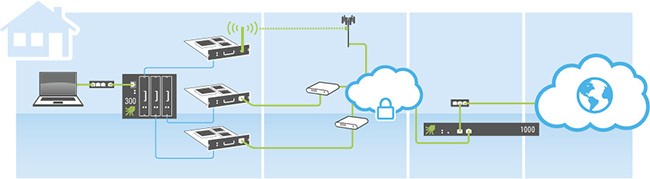
\includegraphics[width=1\textwidth]{WANB.jpg}
    \caption[WANB]{Multi-WAN Bonding Konzept}%[\cite{WANB}]
\end{figure}
Im Vergleich zu einer Normalen Verbindungsmethode handelt es sich beim Multi-Wan Bonding um eine Art von VPN Tunnel. Datenpakete laufen nicht wie gewöhnlich direkt über eine Leitung sondern werden beim betreten des VPN Tunnels von einer Software oder Hardware Multi-Wan Lösung auf mehrere Leitungen aufgeteilt. Dieses Aufteilen alleine ist jedoch noch nicht ganz ausreichend. Um im Endeffekt wieder eine Verbindung zu haben die sich auch verwenden läst ist es Notwendig diese Aufgeteilten Datenpakete wieder zusammen zu führen. Bedeutet es gibt einen Entfernten Endpunkt der als Proxy fungiert. Dieser Endpunkt empfängt die Datenpakete die über die verschiedenen Verbindungen hinausgesandt wurden und setzt diese wieder zu einem Datenstrom zusammen. Damit stellt er das Ende des VPN Tunnels dar. 
\\\\
Es kommt durch das Tunneln selbstverständlich zu einem kleinen Datenüberhang im vergleich zu einer direkten Verbindung da Metadaten zur Steuerung des VPN Tunnels benötigt werden. Oft werden übertragene Daten im Tunnel auch verschlüsselt.
\\\\
Da die Daten, wie bereits erwähnt, über verschiedene Verbindungen übertragen werden, die sich auch in ihrer Stabilität, Geschwindigkeit und Übertragungszeit stark unterscheiden können, muss laufend darauf geachtet werden den Datenstrom entsprechend den aktuellen Leistungs charakteristika der einzelnen Tunnel Datenströme aufzuteilen. Dies geschied vollkommen automatisch durch die verwendete Multi-Wan Bonding Lösung und erfordert kein manuelles eingreifen durch den Anwender.

\subsection{Unterschied zu Load Balancing}
Auch beim Load Balancing werden wie beim Multi-Wan Bonding mehrere WAN Verbindungen verwendet. Die auch im gleichen maße vielfältig sein können.
\\\\
Der entscheidende Unterschied zum Multi-Wan Bonding ist das hier das Aufteilen auf Session-Ebene stattfindet. Hier werden Sessions einfach über den WAN Zugang laufen gelassen der gerade am meisten Ressourcen frei hat. Beim Wan Bonding hingegen wird auf Datenpaket Ebene aufgeteilt. Das aufteilen auf Session-Ebene bringt Vorteile aber auch einige Nachteile.
\paragraph{Load-Balancing Vorteile:}
\begin{enumerate}
    \item Es wird kein entfernter Endpunkt benötigt.
    \item Es gibt keinen Datenüberhang bei der Verbindung.
    \item Ping ist besser aufgrund eines verringertem Verarbeitungsaufwandes. 
\end{enumerate}
\paragraph{Load-Balancing Nachteile:}
\begin{enumerate}
    \item Bandbreite wird nicht gebündelt.
    \item Fällt eine der WAN Verbindungen aus werden auch alle Sessions die über diese Verbindung laufen unterbrochen.
    \item Die Stabilität ist schlechter.
    \item Sessions haben verschiedene IP-Adressen je nach verwendeter WAN Verbindung.
\end{enumerate}


\section{RESTful API}
\section{Network Address Translation (NAT)}
NAT (Network Address Translation) dient im Grundlegenden zur Verbindung zweier getrennter Netzwerke. Im häufigsten Fall zwischen dem Internet und ein einem lokalen Netzwerk. Der größte unterschied zum normalen Routing ist dabei, dass das lokale Netzwerk mit seinen IP-Adressen, im Internet bzw. dem außerhalb liegenden Netzwerk nicht registriert ist. Dies hat natürlich auch zur folge, dass IP-Adressen im lokalen Netzwerk nicht vom äußeren Netzwerk aus erreichbar sind. 
\subsection{Wie funktioniert NAT?}
Wie der Name Network Address Translation bzw. zu Deutsch Netzwerkadressübersetzung schon sagt, werden dabei die nicht unbedingt global eindeutigen IP-Adressen des internen Netzwerks auf eine oder mehrere Adressen im größeren Netzwerk übersetzt. Dies geschieht normal durch ein einzelnes Gerät z.b. einem Router. Dieser Router besitzt sowohl im lokalen unregistriertem Netzwerk eine IP-Adresse als auch im größerem Netzwerk.
\\\\
Erreicht den Router nun ein Datenpaket vom lokalen Netzwerk welches für eine IP-Adresse bestimmt ist die, nicht im lokalen Netzwerk liegt, so leitet er dieses Paket in das äußere Netzwerk weiter. Da die IP-Adressen vom lokalen Netzwerk im äußerem Netzwerk jedoch nicht bekannt sind hätte nun der Empfänger im äußerem Netzwerk keine möglichkeit zu Antworten. Um dieses problem zu lösen kommt nun der eigentliche NAT vorgang zum tragen. 


\newpage
\begin{figure}[h]
    \centering
    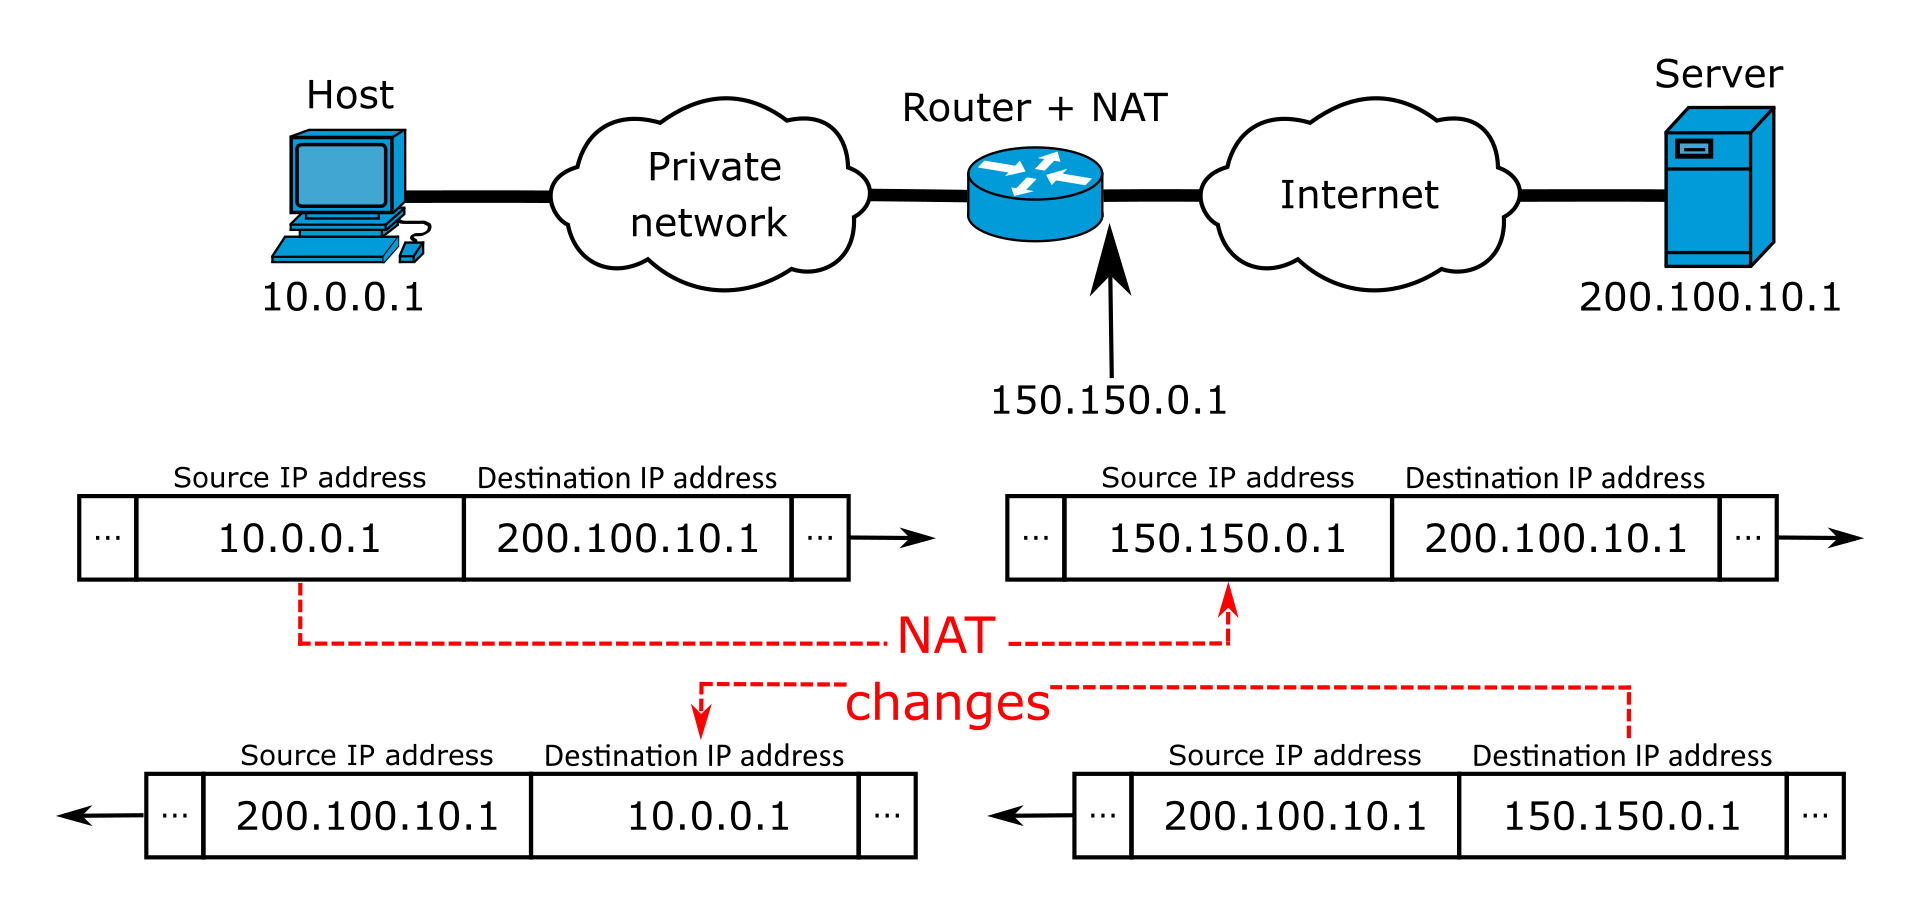
\includegraphics[width=1\textwidth]{NAT1.png}
    \caption[NAT1]{NAT Konzept}%[\cite{NATi1}]
\end{figure}
Der Router der als mittelsmann zwischen den Netzwerken agiert tauscht die Absenderadresse im IP-Header des lokalen Packets gegen seine eigene im äußeren Netzwerk registrierte IP-Adresse aus. Dadurch ist es nun einem Host im äußeren Netzwerk möglich auf das Datenpaket zu Antworten. 
\\\\
Kommt nun eine Antwort bei unserem Router an wird die Ziel IP-Adresse gegen die des ursprünglichen Anfragestellers aus dem lokalen Netzwerk ausgetauscht um im lokalen Netzwerk zugestellt werden zu können.
\subsection{NAT Übersetzungs Tabelle}
Woher weiß nun unser Router für welchen Host im lokalen Netzwerk die Antwort aus dem äußeren Netzwerk bestimmt war? 
\begin{figure}[h]
    \centering
    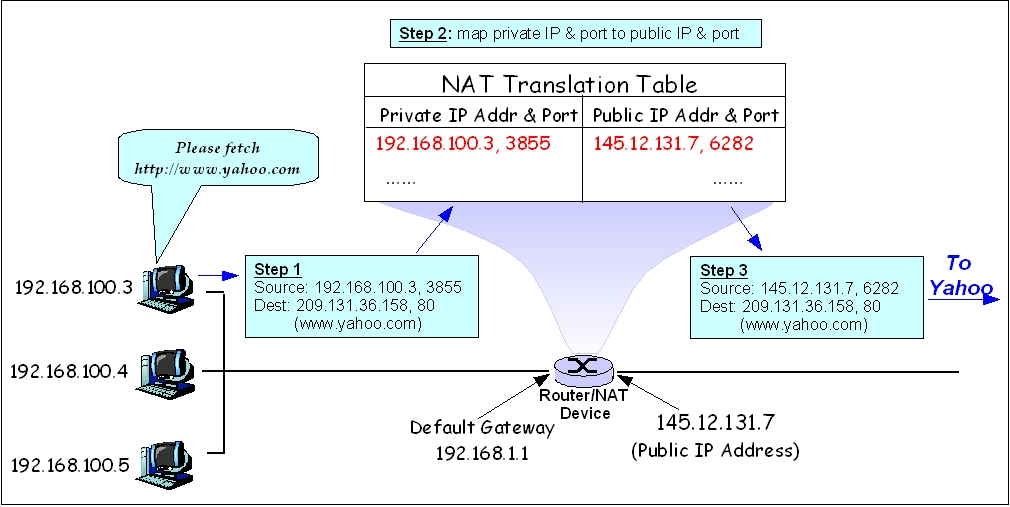
\includegraphics[width=1\textwidth]{NAT2.jpg}
    \caption[NAT2]{NAT Übersetzungs Tabelle}
\end{figure}
Beim Absenden der Anfrage durch den lokalen Host merkt sich der Router in der sogenannten NAT Tabelle den ursprünglichen Port und lokale IP-Adresse, bevor er im NAT Prozess diese durch einen eigenen gewählten Port und eigene registrierte IP-Adresse im größerem Netz ersetzt, welche er ebenfalls in die Tabelle einträgt. 
Kommt nun eine Antwort auf genau diesen äußeren Endpoint (äußere IP-Adresse und gewählter Port vom NAT Prozess) so holt sich der Router aus der NAT Tabelle einfach die ursprüngliche Absender Adresse und Port und setzt diese im empfangenen Antwortpaket als Zieladresse und Zielport ein. 
\subsection{NAT und OSI Schichten}
Da der NAT vorgang auch einen Port benötigt können wir schnell sehen das NAT auf OSI Schicht “4 Transport” arbeitet. Das ist natürlich nicht ganz optimal da es auf einer so hohen schicht relativ lange dauert die Pakete umzuschreiben und weiterzuleiten. Heutzutage werden schon normale Schicht 3 router vermieden und sogut es geht auf Schicht 3 switches gesetzt. NAT kann mit seinem Operationen auf Schicht 4 schon als sehr langsam angesehen werden im verhältnis zu den anderen häufig durchgeführten Netzwerkoperationen wie Switching und Routing.

\subsection{NAT und Ping (ICMP)}
Nicht alle Anwendungen verwenden zwangsläufig Ports und damit Schicht 4. Ping ist so ein beispiel. Ping arbeitet nur auf OSI Layer 3 und arbeitet mit dem ICMP (Internet Control Message Protocol). Wie kann hier nun korrekt NAT Angewandt werden? Würden wir den Port einfach weg lassen in der NAT Tabelle und stattdess nur nach dem Protokoll und Zieladresse gehen gebe es spätestens dann ein Problem wenn 2 Hosts aus dem lokalen Netzwerk gleichzeitig den selbst Host im äußerem Netzwerk anpingen. Es würde dann immer nur der Host im lokalen Netz die Antwort bekommen der zuletzt einen Ping hinaus gesendet hat. 
\\\\
Damit dies nicht passiert wird bei ICMP auf etwas anderes als den Port geachtet. Nämlich auf die ICMP Query ID, diese ID wird im NAT Prozess wie der Port bei TCP, UDP Paketen behandelt. RFC 3022 schreibt dazu im Punkt 4.1 “ICMP header in ICMP Query packets must also be modified to replace the query ID and ICMP header checksum.” - %\cite{NAT1}

\subsection{NAT in zusammenarbeit mit Routing}
NAT alleine wird kaum eingesetzt. Normal passiert dies sogut wie immer im zusammenhang mit einem Router. Was geschieht also zuerst? Wird zuerst NAT Angewendet oder zuerst gerouted?
\\\\
Das hängt ganz davon ab ob es sich um Pakete von dem lokalen Netzwerk für das äußere Netzwerk handelt oder ob es äußere Pakete sind die in unser lokales Netzwerk wollen.
Im ersten Fall, wenn Pakete unser lokales Netzwerk verlassen, wird NAT erst kurz vor dem verlassen des Netzwerkadapters auf das Datenpaket angewendet. 
\\\\
Beim zweiten Fall, wenn ein Paket von außerhalb in unser lokales Netzwerk möchte, wird direkt nach dem eingehen beim Netzwerkadapter NAT angewandt und danach erst gerouted. Dies ist so notwendig da bei NAT die Zieladresse zu einer sich im lokalen Netzwerk befindenden Adresse geändert wird. Es darf also nicht zuvor gerouted werden da dies mit der falschen IP-Adresse geschehen würden. Dieses Problem würde noch größer werden wenn es mehrere lokale Netzwerke gibt.

\subsection{NAT ist eine Notlösung}
Pv4 ist schon lange veraltet und sollte schon längst durch IPv6 abgelöst werden. IPv4 wurde nur noch nicht abgelöst weil ein großteil aller Internet Anwendungen immer noch IPv4 verwenden. Da ein harter umstieg auf IPv6 aber damit auch bedeuten würde das ein großteil aller aktuellen Anwendungen nicht mehr Funktionieren würden, kommt dies nicht in Frage. Auch heute noch werden die meisten Anwendungen für IPv4 geschrieben. Ein Grund dafür ist dass die meisten Entwickler mit IPv4 besser vertraut sind und ein weiterer Grund ist das immer noch nicht alle Internetnutzer eine IPv6-Adresse bekommen.
\\\\
Das große Problem mit IPv4 ist die Anzahl an maximal verfügbaren IP-Adressen. Es gibt einfach nicht mehr genug für die Menge an Geräten die das Internet verwenden. 
Hier kommt nun NAT ins Spiel. NAT ermöglicht es viele unregistrierte Netzwerke zu haben die trotzdem zugang zum Internet haben. Die IP-Adressen in diesen unregistrierten Netzwerken müssen auch nicht eindeutig sein, es kann viele kleine Netzwerke geben die die selben IP-Adressbereiche verwenden und mittels NAT mit dem Internet verbunden sind.
\\\\
Deswegen ist es schon lange Standard geworden das private Internetnutzer von Ihrem ISP einen NAT Router bekommen. So erhält der ganze Haushalt nur eine IP-Adresse und alle Geräte die der Kunde mit dem Router verbindet sind nur im LAN und haben durch den NAT Router nach außen ins das Internet nur die IP-Adresse des Routers. 
\\\\
Bei LTE Routern geht dies sogar noch einen Schritt weiter. Da man nicht jedem Mobiltelefon eine eigene IP-Adresse geben kann wird bei den meisten Sendemasten schon NAT angewendet. Verwendet man nun einen LTE Router für seinen Haushalt hat man schnell doppeltes NAT. Einmal beim Sendemasten und nochmal im eigenen Haus. Dies sorgt für eine Reihe an Problemen die im nächsten Thema vorgestellt werden. 

\subsection{Probleme durch NAT}
NAT bringt auch einige Probleme mit sich. Wie wir bereits beschrieben haben wird ein eintrag in der NAT Tabelle nur gemacht wenn wir zuerst ein Datenpaket hinaus gesendet haben. Bedeutet das ein Endpoint der sich hinter einer NAT Wall befindet nicht aus dem Internet erreichbar ist. Möchte man also einen Server der öffentlich erreichbar ist hinter einer NAT Wall betreiben muss man auf sogenanntes Port Forwarding zurückgreifen. Dabei wird ein Datenpaket für einen bestimmten Port immer zu einem bestimmten Host hinter der NAT Wall weitergeleitet. Alleine wäre das auch noch kein allzu großes Problem, doch sobald es wie in dem LTE Fall doppeltes NAT gibt und wir keinen zugriff auf eine der NAT Router haben ist auch Port Forwarding nicht mehr möglich, dies ist fast immer der Fall wenn man einen LTE Router als normal Anwender verwendet.
\\\\
Auch bei unserer Diplomarbeit stellt unser Server eine zweite NAT Wall dar. Was es Endbenutzern die nicht selbst den NetShare Server betreiben nicht möglich macht Server über NetShare zu hosten die öffentlich zugänglich sein sollen.